\section{物联网设备的认证与授权}
\label{protocol_security}

在物联网环境下,海量终端设备以其微型化、低成本、泛在化的特点为数字世界和物理世界提供了交互的桥梁。一旦设备被非法使用,轻则泄露用户隐私,重则瘫痪整个网络。因此如何合法合规地利用这些终端设备对于物联网安全来说至关重要。通常而言,物联网中的资源调度需要先经过准入认证和权限分配两个主要步骤。一是准入认证,其主要目的是建立各方的信任关系,可大致分为用户认证和设备认证两部分。当用户发起访问请求时,系统会根据用户提供的密码、口令或生物特征等认证凭证,与数据库中预存信息进行匹配以判断是否为合法用户。而接入网络中的设备认证过程也与此相仿,需要设备提供软件指纹或硬件指纹以建立连接。二是权限分配,主要是对资源进行合理的调度管理。在完成用户与设备认证后,系统会根据预存信息对合法接入的用户和设备划分相应权限并分配资源,并防止用户与设备的非法接入和未授权行为的发生。目前物联网中隐私泄露问题多发于接入非法用户和设备,或是非法访问资源,本节将围绕这两个方向进行详细介绍。


\subsection{权限管理与隐私威胁}
\label{common_security}

物联网设备种类繁多,其中智能手机是用户最为依赖和使用最频繁的一类设备。智能手机为了丰富的功能而集成了大量传感组件,导致其面临物联网设备中最为复杂的权限管理挑战,因此在这一节我们以智能手机为代表,讨论物联网设备的权限管理问题。

智能手机上常常部署有大量与用户隐私密切相关的传感器,例如摄像头、麦克风、GPS传感器等等。若不限制应用程序对这些传感器的访问,恶意应用程序将可以轻而易举地获取用户的隐私信息。另一方面,某些敏感的行为,例如开机自启动、在其他应用程序上层显示内容、监控屏幕点击位置、访问通讯录和短信等等,若不加限制,也将会极大地扰乱移动平台的软件生态。

以目前最为流行的Android系统为例,Android早在1.0版本时就已经引入了权限管理机制。不过早期的Android系统仅仅可以做到在应用程序安装时提示用户该应用申请的权限有哪些。图\ref{fig:android5}展示了在Android 5.1操作系统上安装应用程序的效果。对于权限索取不合理的应用程序,用户除拒绝安装外,并无其他选择。随着移动互联网和人工智能技术的飞速发展,软件厂商开始通过大数据分析的手段来了解用户的个人喜好,从而针对性地给予广告推荐,这需要大量的用户隐私信息作为基础。另一方面,也有一些厂商凭借其在市场上的垄断优势,强制用户接受其不合理的权限索取。从这些变化来看,早期的权限管理机制对用户隐私的保护作用就十分有限了。


\begin{figure}[H]
	\begin{center}
		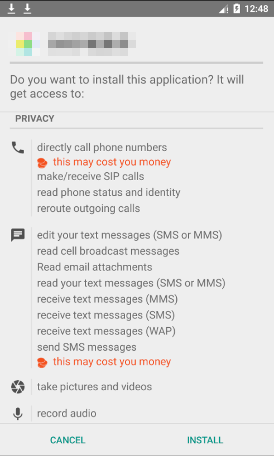
\includegraphics[width=0.3\columnwidth]{Chapter14/graph/android5.png} \\
	\end{center}
	\vspace{-10pt}
	\caption{Android 5.1 下安装应用程序} \label{fig:android5}
	\vspace{-10pt}
\end{figure}

为了解决这些问题,Android操作系统在6.0版本中引入了\textcolor{myblue}{\textbf{运行时权限}}(Runtime Permission)。这意味着用户可以在应用程序运行时对其敏感行为进行拦截。这种机制大大提高了权限管理的灵活性,一定程度上缓解了移动平台上权限滥用的局面。

谷歌公司最新开发的Android 12 当中还引入了``隐私信息中心''这一功能,以便直观地呈现应用程序索取隐私信息的情况。如图\ref{fig:android12}所示,用户可以查看最近有哪些程序访问了摄像头、麦克风以及地理位置信息。这一功能进一步加强了权限管理的约束力,对规范应用程序的隐私获取行为有一定的帮助。

\begin{figure}[H]
	\begin{center}
		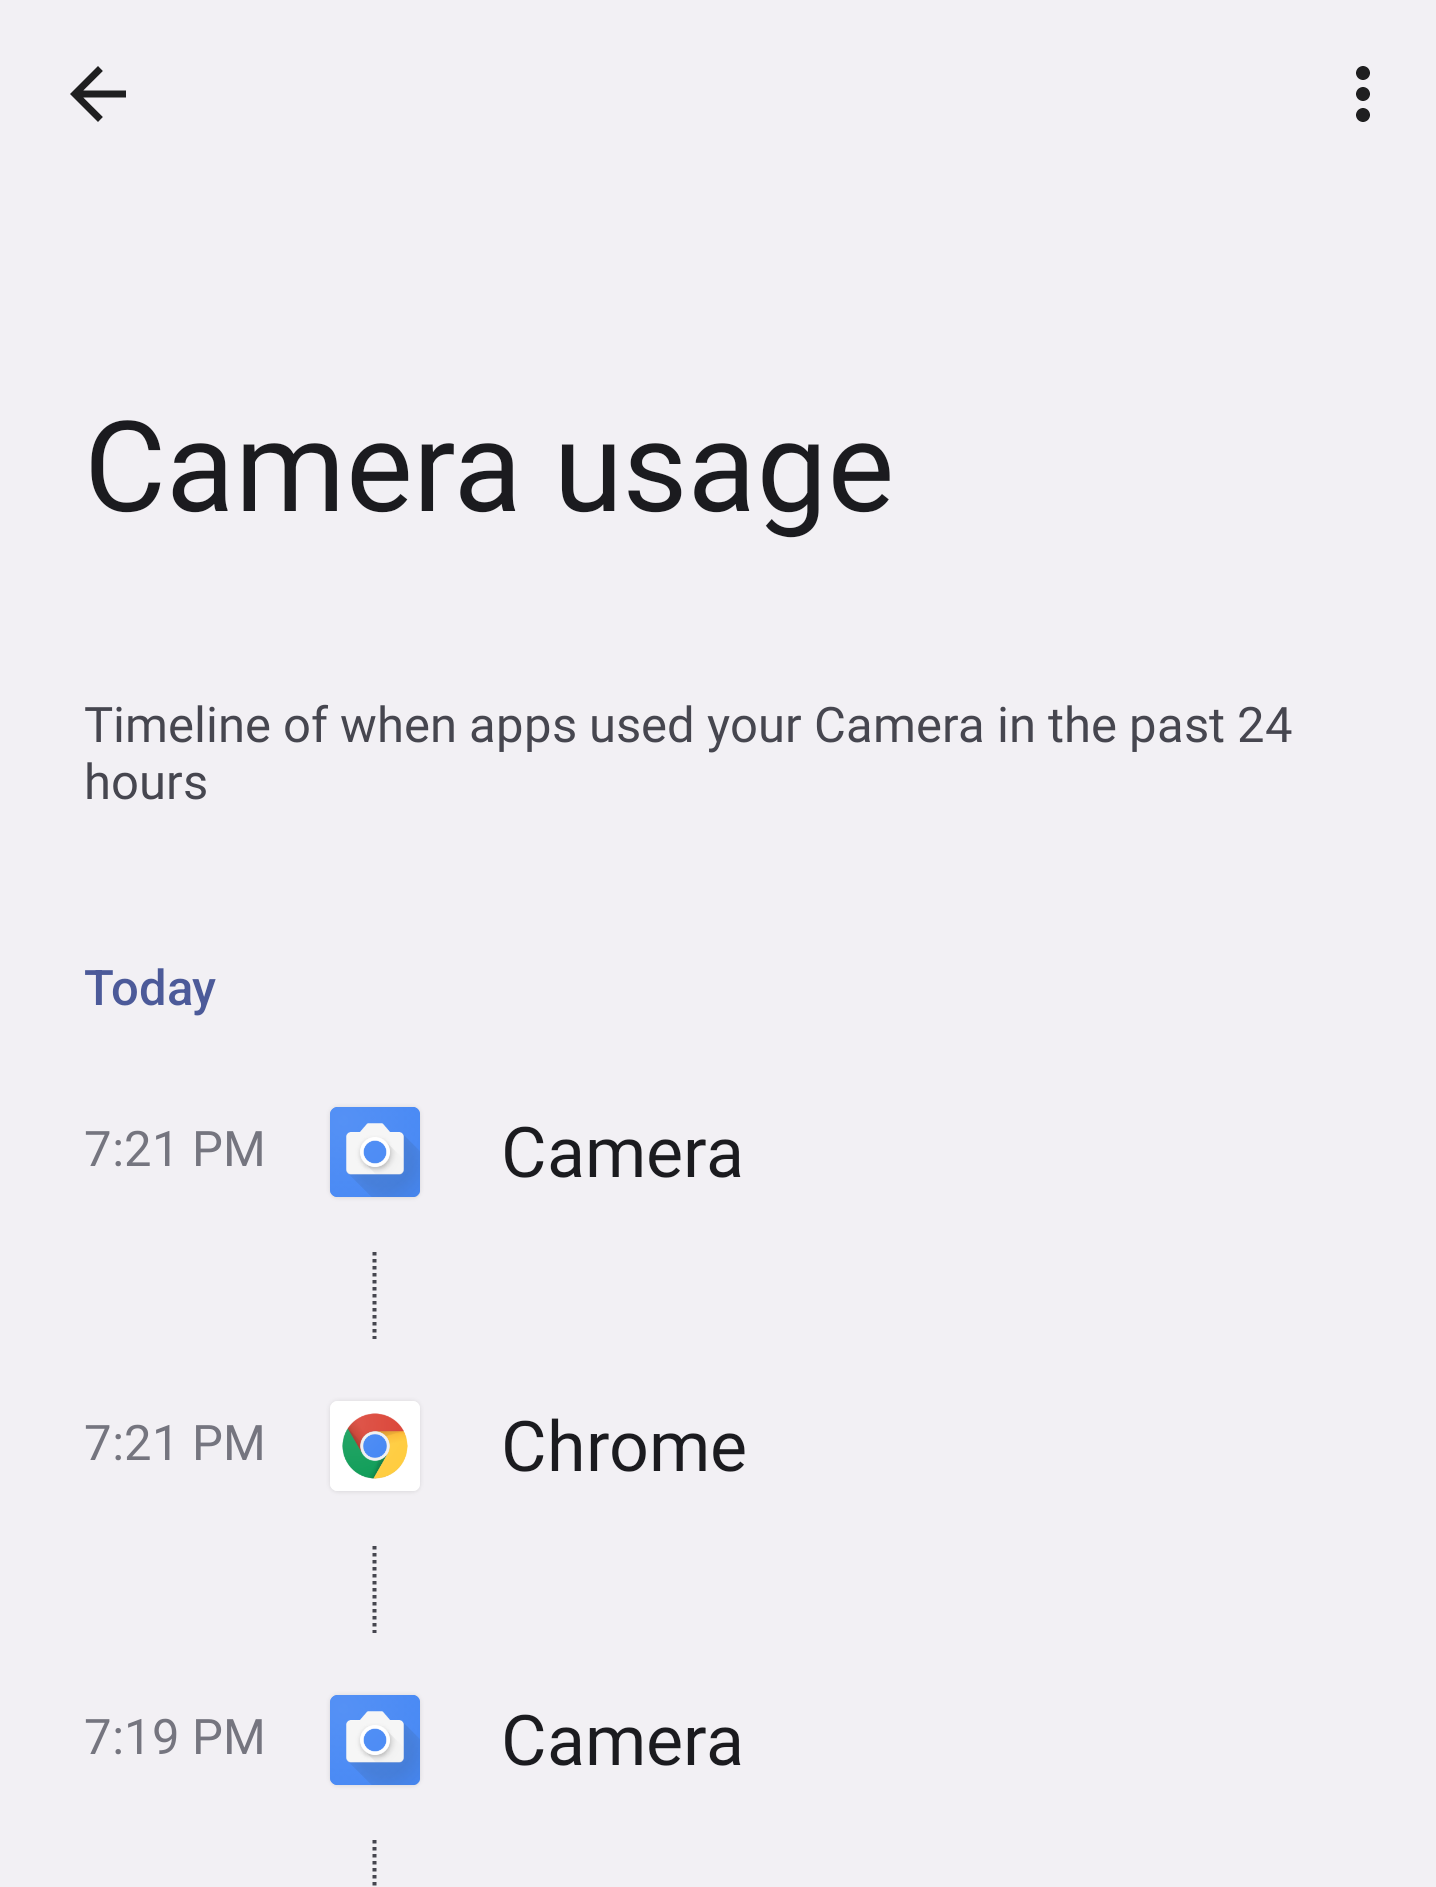
\includegraphics[width=0.3\columnwidth]{Chapter14/graph/android12.png} \\
	\end{center}
	\vspace{-10pt}
	\caption{Android 12 下的隐私信息中心} \label{fig:android12}
	\vspace{-10pt}
\end{figure}


然而,最近的一些研究工作表明,权限管理功能的作用仍是相当有限的。\cite{userbehavior}当中指出,对于不合理的权限索取,仅有不到一半的用户选择了拒绝。大量的用户认为授权操作较为繁琐,从而选择了``始终允许''。由此可以看出用户的隐私保护意识普遍不强。

更为不幸的是,即使用户有足够强的隐私防护意识,也常常无法避免隐私数据的泄漏。一方面,Android系统的权限管理机制在具体实现上仍存在一些漏洞。攻击者可能通过动态分析等手段\cite{escalation},找到并利用这些漏洞,获取敏感权限。另一方面,攻击者也可以通过相对不敏感的信息来推断用户的隐私信息。例如加速度计,陀螺仪等零权限传感器就可能被利用,来达成跟踪用户,窃听环境声音等目的\cite{sensorid,eavesdrop}。
% 当中通过对Android系统权限管理机制的动态分析,发现了一些实现上的漏洞,恶意软件开发者可能利用这些漏洞获取敏感权限。也有一些工作通过相对不敏感的数据来推断敏感的隐私信息。例如通过零权限传感器(例如加速度传感器、陀螺仪等等)来达成跟踪用户、窃听环境声音等目的。
除此之外,一些软件厂商之间还结成了收集用户隐私信息的联盟,以便互通有无。对于某些业务逻辑确需获取的隐私信息(如语音通话应用程序采集到的语音信息,地图导航应用程序采集到的地理位置信息等等),用户也无从得知软件厂商是否会用作其他用途。

可以看出,随着Android系统的不断迭代,其权限管理功能也日趋完善。但是,它仍然存在着很强的局限性。因此,我们还有必要探索其他技术上或管理上的新机制,以便更好地保护用户的隐私。

\subsection{用户与设备认证}
\label{common_security}

\subsubsection{\textcolor{myblue}{\textbf{1.用户身份认证}}}


用户身份认证是保障通讯网络系统安全的根本前提,其目的在于建立各方的信任关系。在物联网环境中,用户必须通过相应的身份验证机制才能获得系统分配的资源和授予的访问权限,进而取得与设备交互的能力。攻击者也通常将身份认证系统作为集中攻击目标,通过中间人攻击、重返攻击、口令猜测攻击等方式,非法获取数据甚至控制设备实施恶意行为。

目前用户认证方案主要存在以下问题:一是缺乏统一的标准规范,导致优质资源分散,难以树立行业标杆。二是受限于有限的计算能力和存储空间,大部分设备只支持轻量级认证方案。三是随着攻击手段的迭代更新,已有设备未必适用新的安全方案或不能及时更新,需要通过更换设备实现。四是物联网的三层架构与计算机网络七层架构不同,许多计算机网络架构下认证方案的可迁移性不足,需要更有针对性地设计适配的认证方案。五是物联网设备异构化强,不同厂商间的通信协议和操作系统通常不同,需要设计兼容性更强的认证方案。

主流用户身份认证方式可根据认证过程发生的位置大致分为两种:一是本地认证,用户可通过预设密码,使用智能卡等物理外设,以及使用指纹和虹膜等生物信息的方式,和设备中预留密钥进行比对认证;二是联网认证,即通过密码学手段对用户提供的秘钥、口令、生物特征等信息进行加密,再同预留在云服务器或边缘网关中的密钥进行匹配。

上述两种认证方式的支撑技术主要有以下几类:一是基于密码的用户身份认证,即用户提供唯一ID与密码组合同预留组合进行匹配认证。二是基于MAC地址或IP地址等公开信息进行认证,这种方式是将硬件地址或网络地址与用户身份进行绑定,安全性和灵活性都相对较弱。三是基于口令的认证,该方法可分为动态和静态两类:动态口令指用户可通过持有相同的口令生成器或经由其它渠道获取一次一密的口令来完成认证;静态口令指用户使用加密狗、智能卡等存储固定口令的方式进行认证。四是基于生物特征的认证,即利用采集设备对指纹、虹膜或声纹等用户独有的生物特征进行获取,并同特征模板库进行匹配实现认证。目前,基于深度学习的多模态用户认证方案正成为该领域热门研究方向之一。上述四种方式多用于本地认证或联网认证的接入阶段,其主要目的在于根据用户所知、所有或特征信息作为准入凭证,而下述两类技术则更专注于为这些凭证提升可信程度。五是基于区块链技术设计用户认证系统,利用分布式账本抗抵赖的特性提升系统审计能力。六是使用密码学方法提升认证凭证安全性,即利用哈希算法、对称和非对称密码算法对用户提供的认证凭证进行加解密计算,如利用椭圆曲线加密,秘密共享和秘钥分割等方式进行认证。另外,利用量子密码进行用户认证的方式也逐渐成为主要研究方向之一。

目前,现有技术虽具备一定的防护能力,但长远看来,随着传感器种类的丰富与设备数量的激增,物联网环境下的用户认证方案也将面临更艰巨的考验。从现阶段发展状况看,用户身份认证系统大致有如下发展趋势:一是更注重数据安全和隐私保护;二是利用轻量级加密算法实现轻量级认证;三是通过降低计算成本等方式提升认证效率;四是提升对大量节点与海量接入的管理能力,可以更便捷地实现节点纳新;五是提升异构方案适配能力,兼容多平台和多协议,开发友好API;六是机器学习、区块链和量子计算等新技术将进一步推进用户认证系统发展;七是增强系统鲁棒性;八是提升审计能力。

\subsubsection{\textcolor{myblue}{\textbf{2.设备身份认证}}}

用户身份认证至关重要,而互联设备的身份认证也极其重要。在物联网环境中,各设备之间存在大量点对点通信,为了避免指令混乱甚至恶意攻击,设备在执行指令之前必须确保互联设备的真实性。因此,对设备提取设备指纹并进行设备身份认证至关重要。目前,设备指纹主要分为软件指纹和硬件指纹两类。

软件指纹是指人为对设备设定的识别标识,包括:唯一标识密钥(安全令牌)、国际移动设备标识(IMEI)、MAC地址、浏览器指纹等。
其中,唯一标识密钥用于同一网络内设备之间的身份认证,设备可使用该密钥进行安全通信。
国际移动设备标识是一种和设备相关的唯一标识,相当于用户的唯一ID,在通信时通过验证IMEI码即可确认互联设备身份。
同样的,MAC地址是联网设备的一种唯一标识,用于网络配置。因为其唯一性,也常用于设备身份验证。
而浏览器指纹是通过浏览器和Cookie获取设备软硬件设置等信息来识别设备。
以上这些设备指纹都存在一定的安全风险,比如:安全令牌一旦泄露,整个网络通信将不再可信。
IMEI码和MAC地址的篡改也并不困难。
在用户隐私保护意识较强的今天,许多用户会选择关闭Cookie记录,这直接导致浏览器指纹的可靠性大幅降低。
因此,以上软件指纹普遍存在易被篡改、可靠性低等问题,设备认证整体安全性较低。

硬件指纹是指物联网设备硬件与生俱来的一种特性,这种特性存在于每台设备中,且设备之间各不相同。
这种硬件指纹来源于传感器等部件生产的不完美性,验证端可以从传感器采集的数据中提取硬件指纹。
常用的设备硬件指纹有:相机指纹、音频指纹、运动传感器指纹等。
其中,相机指纹是摄像头上的硬件指纹。摄像头最重要的感光元件由几百万个像素点组成,由于生产工艺的不完美性,每个成品的感光元件不可能完全一致,像素点之间细微的透光差异将在拍摄的每张照片中留下痕迹。这种唯一且与生俱来的痕迹称为相机指纹。通过对照片提取相机指纹,就可以判断摄像头所在设备的身份。
音频指纹由麦克风和扬声器组合生成,它们拥有相似的结构,都由磁钢和线圈组成,但每个磁钢与线圈之间的距离存在一定差异,具体体现在播放与录音的结果中。即使播放相同的音频,扬声器输出的声音并不相同。同理,即使在相同距离接收同一声音,不同麦克风收录的内容也有差异。两者组合时,扬声器播放相同音频,麦克风同时录制,就可以得到录音对应的独特频率响应曲线,并作为硬件指纹进行设备认证。
运动传感器主要包括加速度传感器和陀螺仪。同样因为生产的不完美性导致个体差异,成品件对相同运动的响应存在差异。因此,在相同震动情况下,不同传感器采集到的震动信息不同,可以作为设备硬件指纹进行身份认证。
这类硬件指纹不由人工设定,没有重复性也无法篡改与伪造,属于安全性较高的设备验证指纹。
 
 
\subsection{前沿研究}
物联网中的资源调度要经过权限管理和认证两个步骤。在这一节中,首先介绍权限管理相关的前沿工作,然后说明近年来学术界在设备和用户认证方面的研究成果。

近年来许多研究表明,仅依赖权限管理并不能完全解决物联网的安全和隐私问题。现有的权限管理机制依据传感组件权限的敏感程度经验性地将其划分为高权限(相机、麦克风、扬声器)及零权限(加速度计,陀螺仪和磁力计等)两类。仅有少量的研究是利用高权限传感组件窃取用户个人隐私的\cite{yu2016writinghacker,song2016my,yu2019indirect,schlegel2011soundcomber,guri2017speake},低权限传感器的隐私泄露问题是近年来国内外学者关注的热点之一。许多工作都是利用智能设备内置的陀螺仪或加速计来采集震动信号,识别乃至重建语音信息\cite{michalevsky2014gyrophone,zhang2015accelword,feng2017continuous,anand2018speechless,Ba2020Learning}。除零权限运动传感器外,一些研究还分别探索了其它异构传感组件用于窃取语音信息的可能性,例如高帧率摄像机\cite{davis2014visual}、激光雷达\cite{sami2020spying}、振动马达\cite{2016Listening}。除音频信息以外,还可以利用零权限传感器推断用户输入的数字及文本等敏感信息\cite{Xu2012Taplogger,Miluzzo2012Tapprints,Owusu2012Accessory,Cai2011TouchLogger}、运动行为\cite{kwapisz2011activity,shoaib2013towards}以及位置信息\cite{han2012accomplice}。

设备和用户认证是物联网是极其关键的一环,一直以来深受国内外学者关注。对于设备认证而言,由于硬件其本身物理不可克隆的特性,硬件指纹成为设备认证的一大研究热点。例如,部分工作利用扬声器和麦克风的听觉指纹来进行设备认证\cite{Das2014Do,Zhou2014Acoustic,Chen2015Wireless},同时智能设备内置相机的光响应非均匀性也被作为硬件指纹用于认证\cite{Ba2018ABC}。另外,软件指纹也有较多的研究成果,一些研究围绕轻量的多密钥认证模式展开研究\cite{Hammi2020A,Shah2018Authentication},区块链技术也被用于设备认证\cite{Li2018A}。

对于用户认证而言,近年来大多数研究利用智能设备的传感组件,通过捕捉生物行为特征,实现了连续和隐式的用户身份验证。大多数研究利用加速度计、陀螺仪和传感器来寻找用户的行为模式,从而进行用户认证,例如挥舞手势\cite{Hong2015Waving}、自由手势\cite{Meidan2017Detection}、拾起动作(即拿起手机并举起手机接听)\cite{Francois2010Machine}、手指按压屏幕\cite{Liu2017Vibwrite}。除此之外,眼睛移动的模式也被用于识别用户身份\cite{Zhang2018VR,Song2016Phone}。